\chapter{One Euro filter}

Le One Euro filter est un algorithme permettant permettant de filtrer un tracé. Nous allons donc nous servir de cet algorithme pour pallier le bruit obtenu dans les données récupérées de la Kinect.

\section{Présentation}
 Le One Euro filter \cite{oneeuro} est un filtre développé par l'INRIA et dont l'implémentation dans certains langages dont le C++ est disponible sur internet. Celui-ci est un filtre passe-bas, c'est à dire que les hautes frequences sont eliminées. Cela permet ainsi d'éliminer les tremblements du curseur.
	
\section{Implémentation}

Une implémentation en C++ du \textit{One Euro Filter} est disponible sur internet.

%le code ou on filtre dans le Ktrack

Il a été décidé de faire le traitement des données coté client et non serveur pour que l'application puisse desactiver le filtrage si nécessaire, et utiliser en paralléle les données filtrées et les données bruitées.
Une fois le filtre utilisé une latence entre le moment où le mouvement est effectué et le déplacement du curseur est apparue. Ceci étant gênant pour une application de dessin, nous avons dù régler les paramètres du One Euro Filter pour réduire cette latence.

\section{Réglage}

Le réglage du One Euro Filter est une partie importante du projet puisqu'elle affecte l'expérience de l'utilisateur. Il nous faut corriger au mieux le signal que l'on reçoit de la Kinect sans pour autant causer une gêne d'utilisation. Nous avons observé les exemples du One Euro Filter \cite{oneeurodemo}, et nous avons modifié nos paramètres de filtre.

Nous avons fait tester l'application par plusieurs personnes et ajuster les paramètres de filtre en fonction de leurs retours d'utilisation.

Nous obtenons finalement une utilisation très fluide et réactive avec un traitement du signal efficace. 

Voici un aperçu du résultat de l'application du filtre:

\begin{figure}[!ht]
	\center
	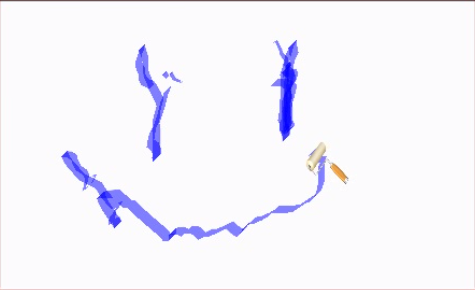
\includegraphics[scale=0.6]{image/bruit.png}
	\caption{Dessin d'un smiley, bruitage trop important}
	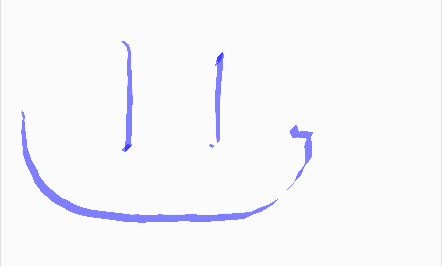
\includegraphics[scale=0.6]{image/nonbruit.png}
	\caption{Dessin d'un smiley, bruitage réduit par le filtre}
\end{figure}

Compte-tenu du bruit obtenu par une Kinect, il serait très compliqué d'obtenir un résultat de meilleure qualité sans utiliser des paramètres de lissage plus conséquents, combinés avec des algorithmes de prédiction tels que le dead reckoning.